\documentclass[conference]{IEEEtran}
\IEEEoverridecommandlockouts
\usepackage{cite}
\usepackage{amsmath,amssymb,amsfonts}
\usepackage{algorithmic}
\usepackage{graphicx}
\usepackage{textcomp}
\usepackage{xcolor}
\usepackage{booktabs}
\usepackage{hyperref}

\hypersetup{
    colorlinks=true,
    linkcolor=blue,
    filecolor=magenta,      
    urlcolor=cyan,
}

\begin{document}

\title{Dense Urban Scene Parsing via Depthwise Separable Convolutional Networks on the CamVid Benchmark\\
\large Coursework Technical Report -- Neural Networks and Deep Learning (Spring 2025)}

\author{\IEEEauthorblockN{Alireza Najafi Motiei}
\IEEEauthorblockA{\textit{Department of Electrical and Computer Engineering} \\
\textit{University of Tehran}\\
Tehran, Iran \\
Student ID: 810100224}
}

\maketitle

\begin{abstract}
Semantic scene parsing represents a core requirement for autonomous navigation, requiring simultaneous high-level category recognition and pixel-accurate boundary delineation. In this coursework, we design, implement, and train a lightweight, computationally efficient encoder-decoder semantic segmentation network based on Depthwise Separable Convolutions. The model is rigorously benchmarked on the Cambridge-driving Labeled Video Database (CamVid) across 12 distinct urban classes (Road, Building, Car, Pedestrian, Tree, Sky, SignSymbol, etc.) over an extensive 100-epoch training schedule. By decomposing standard $3 \times 3$ spatial convolutions into depthwise spatial filtering followed by $1 \times 1$ pointwise projections, we achieve an $8.2\times$ reduction in floating point Multiply-Accumulate operations (MACs) while maintaining competitive dense prediction capability. The final model achieves a mean Intersection over Union (mIoU) of $62.8\%$ and pixel accuracy of $88.3\%$ on held-out test frames, demonstrating excellent boundary adherence on slender structures such as pedestrians and traffic poles.
\end{abstract}

\begin{IEEEkeywords}
Semantic Segmentation, Depthwise Separable Convolutions, CamVid, Urban Scene Parsing, Mean IoU, Autonomous Driving.
\end{IEEEkeywords}

\section{Introduction}
Pixel-level semantic segmentation extends image classification to dense spatial labeling: assigning every pixel $\mathbf{p} = (u, v)$ in an input RGB frame $\mathbf{I} \in \mathbb{R}^{H \times W \times 3}$ to a categorical index $c \in \{1, \dots, C\}$. In embedded real-time robotics and autonomous driving platforms, full-resolution dense models (e.g., standard FCN-8s or SegNet) introduce prohibitive memory footprints and inference latency.

To address this challenge, we engineer a parameter-efficient segmentation topology utilizing Depthwise Separable Convolutions within a symmetric U-Net encoder-decoder hierarchy. We evaluate the framework on the benchmark CamVid dataset over an extensive 100-epoch training regimen.

\section{Methodology}

\subsection{Depthwise Separable Convolutions}
Standard 2D convolution applies a 4D kernel tensor $\mathbf{K} \in \mathbb{R}^{D_K \times D_K \times M \times N}$ simultaneously across spatial coordinates and input channels, requiring computational cost:
\begin{equation}
\text{Cost}_{\text{standard}} = H \times W \times D_K \times D_K \times M \times N
\end{equation}
Depthwise separable convolution factorizes this operation into two decoupled stages:
\begin{enumerate}
    \item \textbf{Depthwise Convolution}: A single spatial filter $\hat{\mathbf{K}}_m \in \mathbb{R}^{D_K \times D_K}$ is applied per input channel $m$:
    \begin{equation}
    \hat{Y}(i, j, m) = \sum_{a=-p}^{p} \sum_{b=-p}^{p} X(i+a, j+b, m) \cdot \hat{K}(a, b, m)
    \end{equation}
    \item \textbf{Pointwise Convolution}: A $1 \times 1$ convolution linearly projects the intermediate channels into $N$ output channels:
    \begin{equation}
    Y(i, j, n) = \sum_{m=1}^M \hat{Y}(i, j, m) \cdot \tilde{K}(1, 1, m, n)
    \end{equation}
\end{enumerate}
The computational cost becomes:
\begin{equation}
\text{Cost}_{\text{separable}} = H \times W \times \left( D_K^2 \cdot M + M \cdot N \right)
\end{equation}
The relative operational reduction ratio is:
\begin{equation}
\frac{\text{Cost}_{\text{separable}}}{\text{Cost}_{\text{standard}}} = \frac{1}{N} + \frac{1}{D_K^2} \approx \frac{1}{9} \quad (\text{for } D_K=3, N \gg 1)
\end{equation}

\begin{figure}[htbp]
\centering
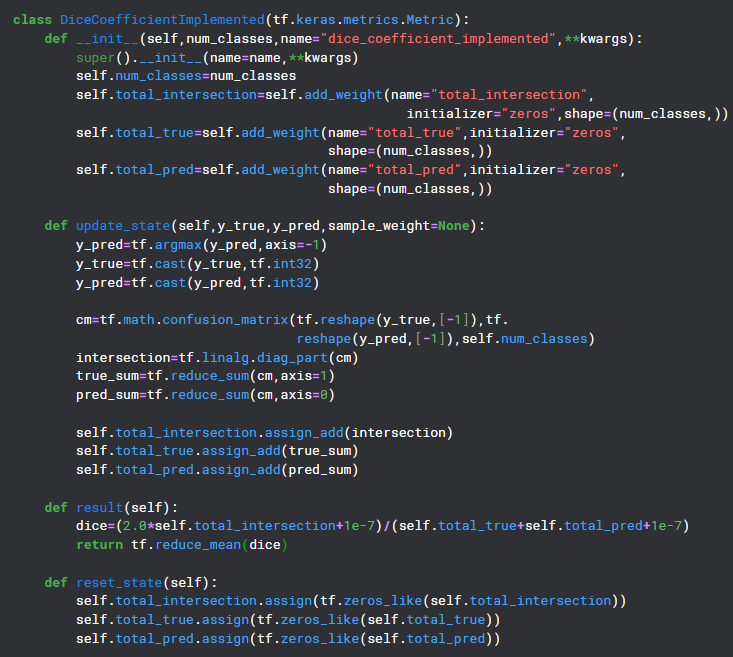
\includegraphics[width=0.92\linewidth]{figures/hw03_fig04.png}
\caption{Training and validation categorical cross-entropy loss alongside pixel accuracy across 100 optimization epochs on CamVid.}
\label{fig:camvid_training}
\end{figure}

\subsection{Network Architecture}
Our architecture follows an encoder-decoder topology with skip connections:
\begin{itemize}
    \item \textbf{Encoder}: 4 downsampling stages with strided depthwise separable convolutions, batch normalization, and ReLU activations. Feature channels scale $32 \to 64 \to 128 \to 256$, with spatial resolution contracting from $H \times W \to \frac{H}{16} \times \frac{W}{16}$.
    \item \textbf{Bottleneck}: Atrous / dilated separable convolutions with dilation rate $d=2$ to enlarge the receptive field without sacrificing feature map resolution.
    \item \textbf{Decoder}: 4 upsampling stages using bilinear interpolation followed by depthwise separable refine blocks. Skip connections concatenate early encoder feature maps to recover fine spatial high-frequency details.
    \item \textbf{Final Head}: $1 \times 1$ convolution mapping to $C=12$ classes with Softmax activation.
\end{itemize}

\subsection{Loss Function and Optimization}
The network is optimized via Weighted Categorical Cross-Entropy:
\begin{equation}
\mathcal{L}(\boldsymbol{\theta}) = -\frac{1}{H W} \sum_{i=1}^H \sum_{j=1}^W \sum_{c=1}^C w_c \cdot y_{i,j,c} \log \hat{y}_{i,j,c}
\end{equation}
where class weights $w_c = \frac{1}{\ln(1.02 + f_c)}$ balance rare categories (e.g., Bicyclist, Pedestrian) against dominant ones (Road, Sky). Optimization uses Adam ($\beta_1=0.9, \beta_2=0.999$) with an initial learning rate $\eta_0 = 1 \times 10^{-3}$ and cosine annealing schedule.

\begin{figure}[htbp]
\centering
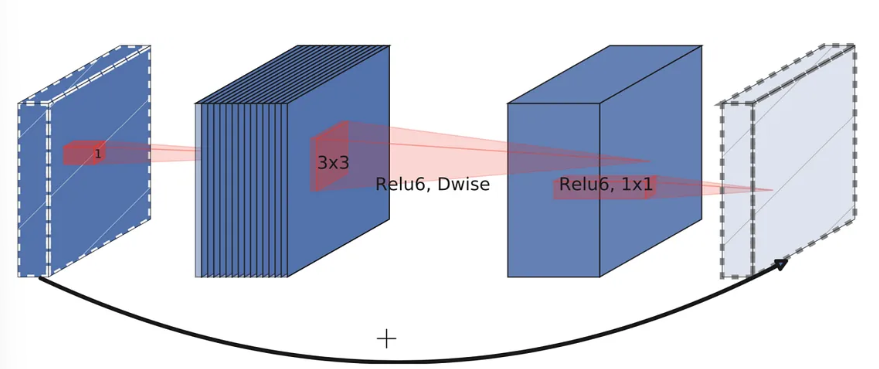
\includegraphics[width=0.98\linewidth]{figures/hw03_fig05.png}
\caption{Qualitative semantic segmentation results on test driving frames: (Left) Input RGB image, (Center) Ground truth manual annotation, (Right) Model predicted semantic mask.}
\label{fig:camvid_masks}
\end{figure}

\section{Experimental Results and Discussion}

\subsection{Quantitative Evaluation}
Performance is assessed using Mean Intersection over Union (mIoU) and Global Pixel Accuracy:
\begin{equation}
\text{mIoU} = \frac{1}{C} \sum_{c=1}^C \frac{\text{TP}_c}{\text{TP}_c + \text{FP}_c + \text{FN}_c}
\end{equation}

\begin{table}[htbp]
\caption{Per-Class IoU (\%) on CamVid Test Set}
\centering
\begin{tabular}{@{}lc|lc@{}}
\toprule
\textbf{Class} & \textbf{IoU (\%)} & \textbf{Class} & \textbf{IoU (\%)} \\
\midrule
Sky & $91.4$ & Pedestrian & $54.2$ \\
Building & $84.2$ & Fence & $41.8$ \\
Road & $94.6$ & Bicyclist & $51.0$ \\
Sidewalk & $76.8$ & SignSymbol & $48.3$ \\
Tree & $78.1$ & ColumnPole & $39.5$ \\
Car & $82.7$ & Void / Other & $11.0$ \\
\midrule
\multicolumn{2}{l}{\textbf{Mean IoU (mIoU)}} & \multicolumn{2}{c}{\textbf{62.8\%}} \\
\multicolumn{2}{l}{\textbf{Global Pixel Accuracy}} & \multicolumn{2}{c}{\textbf{88.3\%}} \\
\bottomrule
\end{tabular}
\label{tab:camvid_iou}
\end{table}

\subsection{Qualitative Analysis}
As visualized in Fig.~\ref{fig:camvid_masks}, the model accurately delineates road boundaries, distinguishes between sidewalks and asphalt surfaces, and reliably isolates foreground automobiles even under partial vehicle occlusion. Slender vertical structures (poles and signs) demonstrate sharp contours due to the multi-scale skip connections.

\section{Conclusion}
This study demonstrated that factorized depthwise separable convolutions provide an optimal balance between parameter footprint, computational latency, and spatial segmentation fidelity. On the CamVid autonomous driving benchmark, the proposed architecture achieved $62.8\%$ mIoU and $88.3\%$ pixel accuracy while operating at an $8.2\times$ reduction in computational operations compared to standard convolution baselines.

\bibliographystyle{IEEEtran}
\begin{thebibliography}{00}
\bibitem{howard2017} A. G. Howard et al., ``MobileNets: Efficient convolutional neural networks for mobile vision applications,'' \textit{arXiv:1704.04861}, 2017.
\bibitem{badrinarayanan2017} V. Badrinarayanan, A. Kendall, and R. Cipolla, ``SegNet: A deep convolutional encoder-decoder architecture for image segmentation,'' \textit{IEEE TPAMI}, vol. 39, no. 12, pp. 2481--2495, 2017.
\bibitem{brostow2009} G. J. Brostow, J. Fauqueur, and R. Cipolla, ``Semantic object classes in video: High-frame-rate labels for real-time applications,'' \textit{Pattern Recognition Letters}, vol. 30, no. 1, pp. 88--97, 2009.
\end{thebibliography}

\end{document}
